\begin{frame}{Results}{Discussion}
    \begin{block}{OC, MSE and mismatch increase}
        Increase in gating intensity tended to increase 
        observation coverage, mean squared error, and data mismatch,
        albeit with case-dependent sensitivities.
    \end{block}
    \vfill
    \def\arraystretch{2}
    \begin{tabular}{rp{0.9\linewidth}}
        $\triangleright$ & Gating reduces posterior variance loss, so increase in coverages, but also MSE and mismatch, are expected as gating intensifies.
    \\
        $\triangleright$ & Egg standard deviations are lesser than Olympus on two accounts:
        reservoir complexity, and ground-truth representativeness. Olympus' ground-truths were somewhat biased.
    \end{tabular}
    \vfill
\end{frame}

\begin{frame}{Results}{Discussion}
    \begin{block}{Mixed effects of localization}
        Localization yielded mixed results: for the Egg and real field cases,
        effects on coverage and MSE were minimal, especially for intense enough gatings,
        while the effect in the Olympus case was drastic.
        %
        % Cumulative distribution plots of the field oil production total suggest 
        % that ground-truths are unbiased in the Egg and real field cases,
        % but somewhat biased for the Olympus case.
    \end{block}
    \vfill
    \def\arraystretch{1.75}
    \begin{tabular}{rp{0.93\linewidth}}
        $\triangleright$ & 
        \textbf{Egg case}:
            narrow FOPT range and roughly uniform sampling of ground-truths leave no ground-truth unrepresented,
            reduced dimentionality help with covariance estimation.
    \\
        $\triangleright$ &
        \textbf{Olympus case}:
            much more complex while also having a much smaller ensemble
            and a lot more features, aggravating covariance estimation.
            Localization was conceived exactly for such situations, so it is not suprising it was effective here.
    \\
        $\triangleright$ &
        \textbf{Real field case}:
            peak complexity and dimentionality, but also ensemble size.
            Localization may have inadequately adjusted, and some features are not well-represented.
    \end{tabular}
\end{frame}

\begin{frame}{Results}{Discussion}
    \begin{figure}[h!]\centering
        \begin{subfigure}{.49\linewidth}\centering
            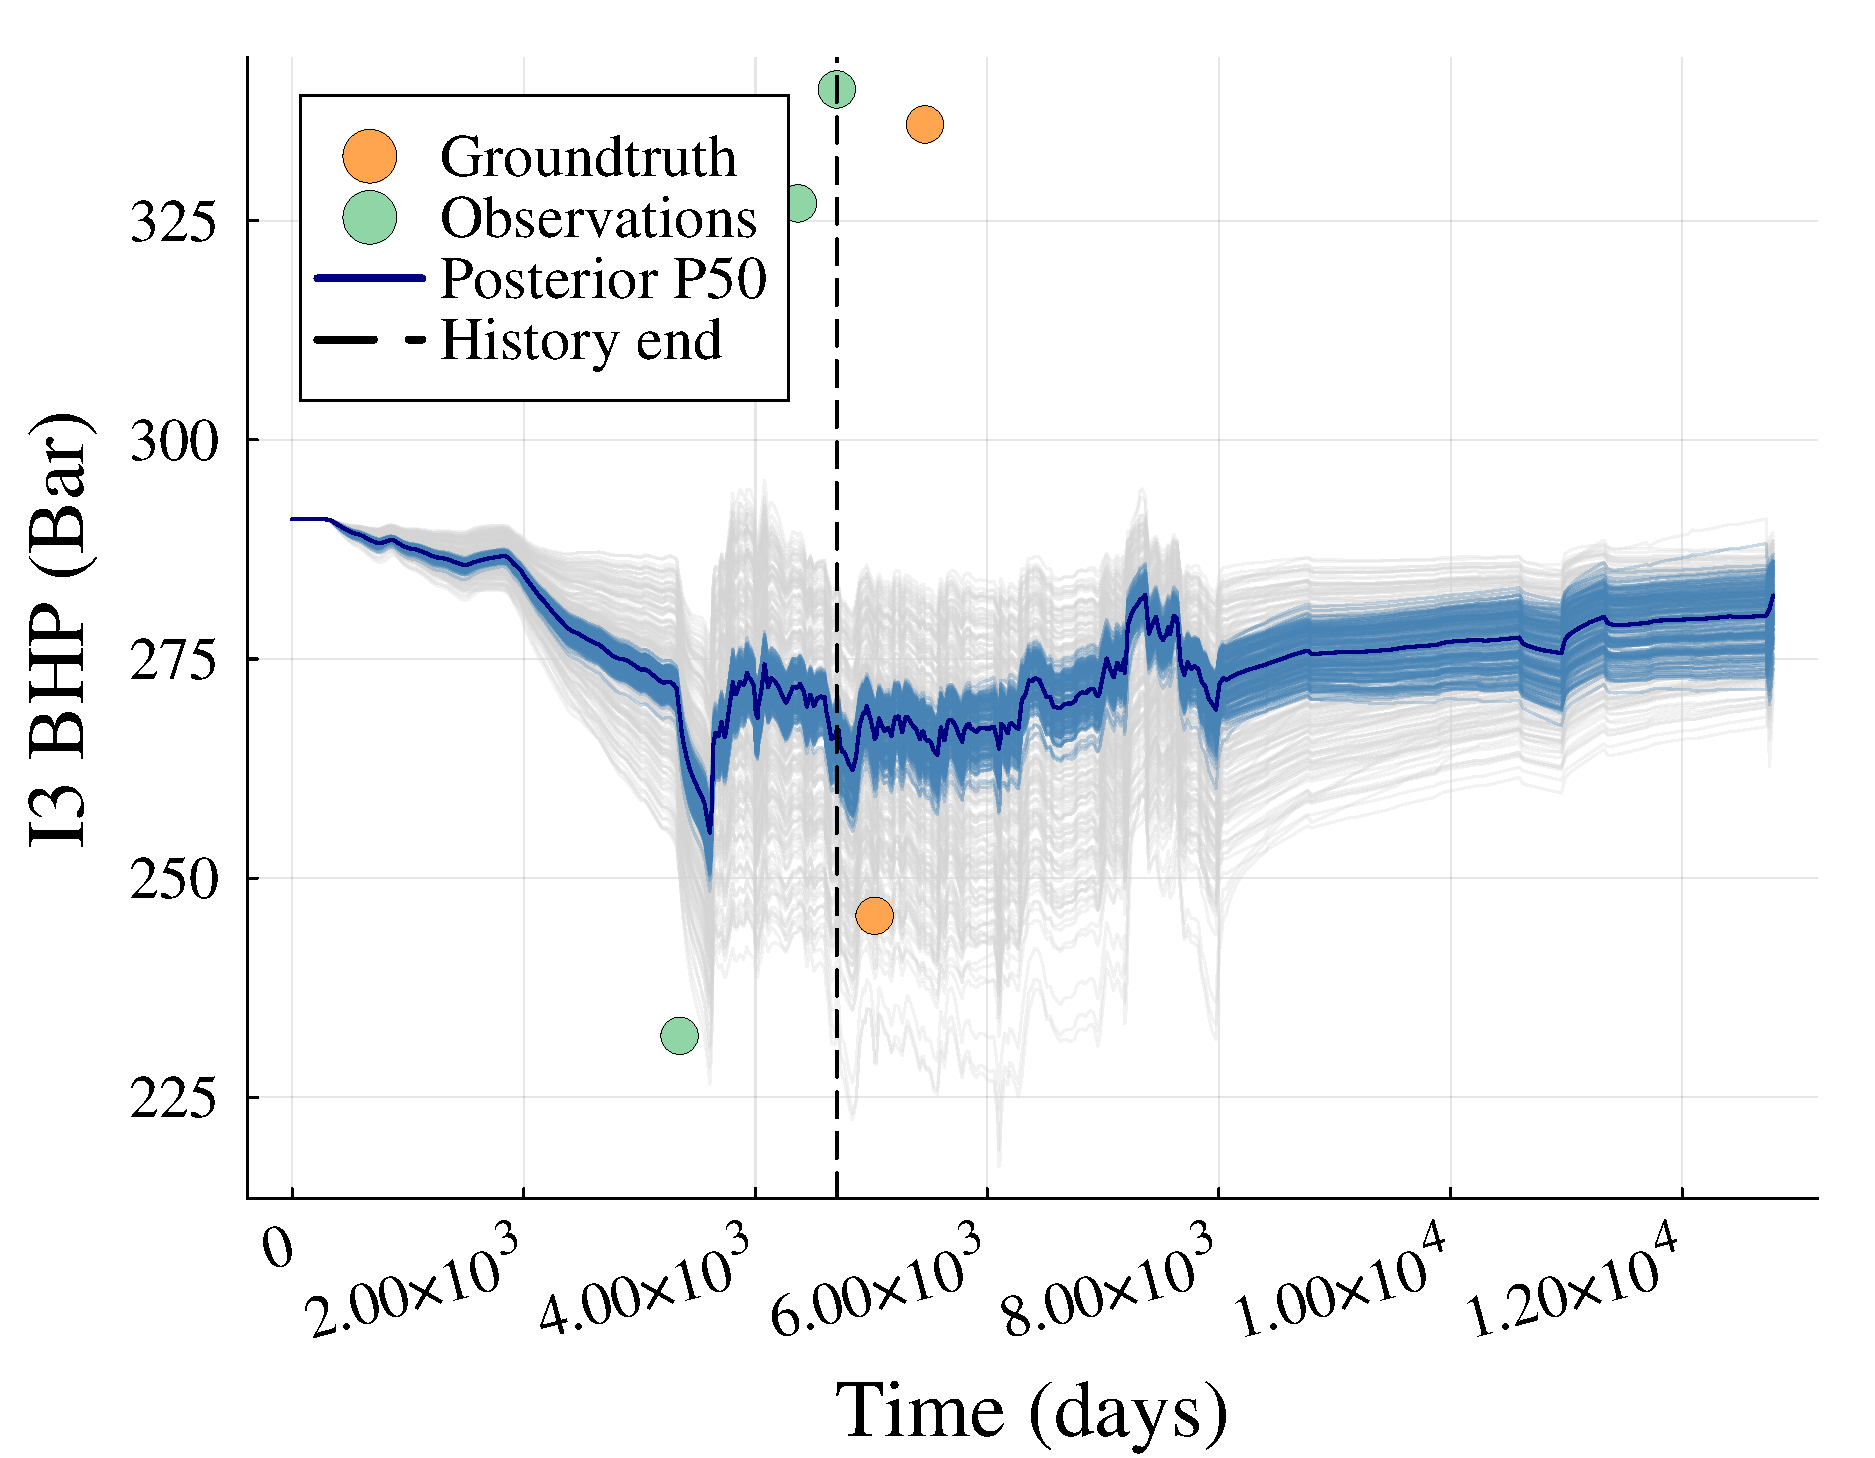
\includegraphics[width=0.775\linewidth]{figures/results/real_field/gt_0/noise_magnitude_0.01/n_iterations_1/localization_false/gating_true/gating_intensity_4.0/WELLS_I3_WBHP.pdf}
        \end{subfigure}  
        \begin{subfigure}{.49\linewidth}\centering
            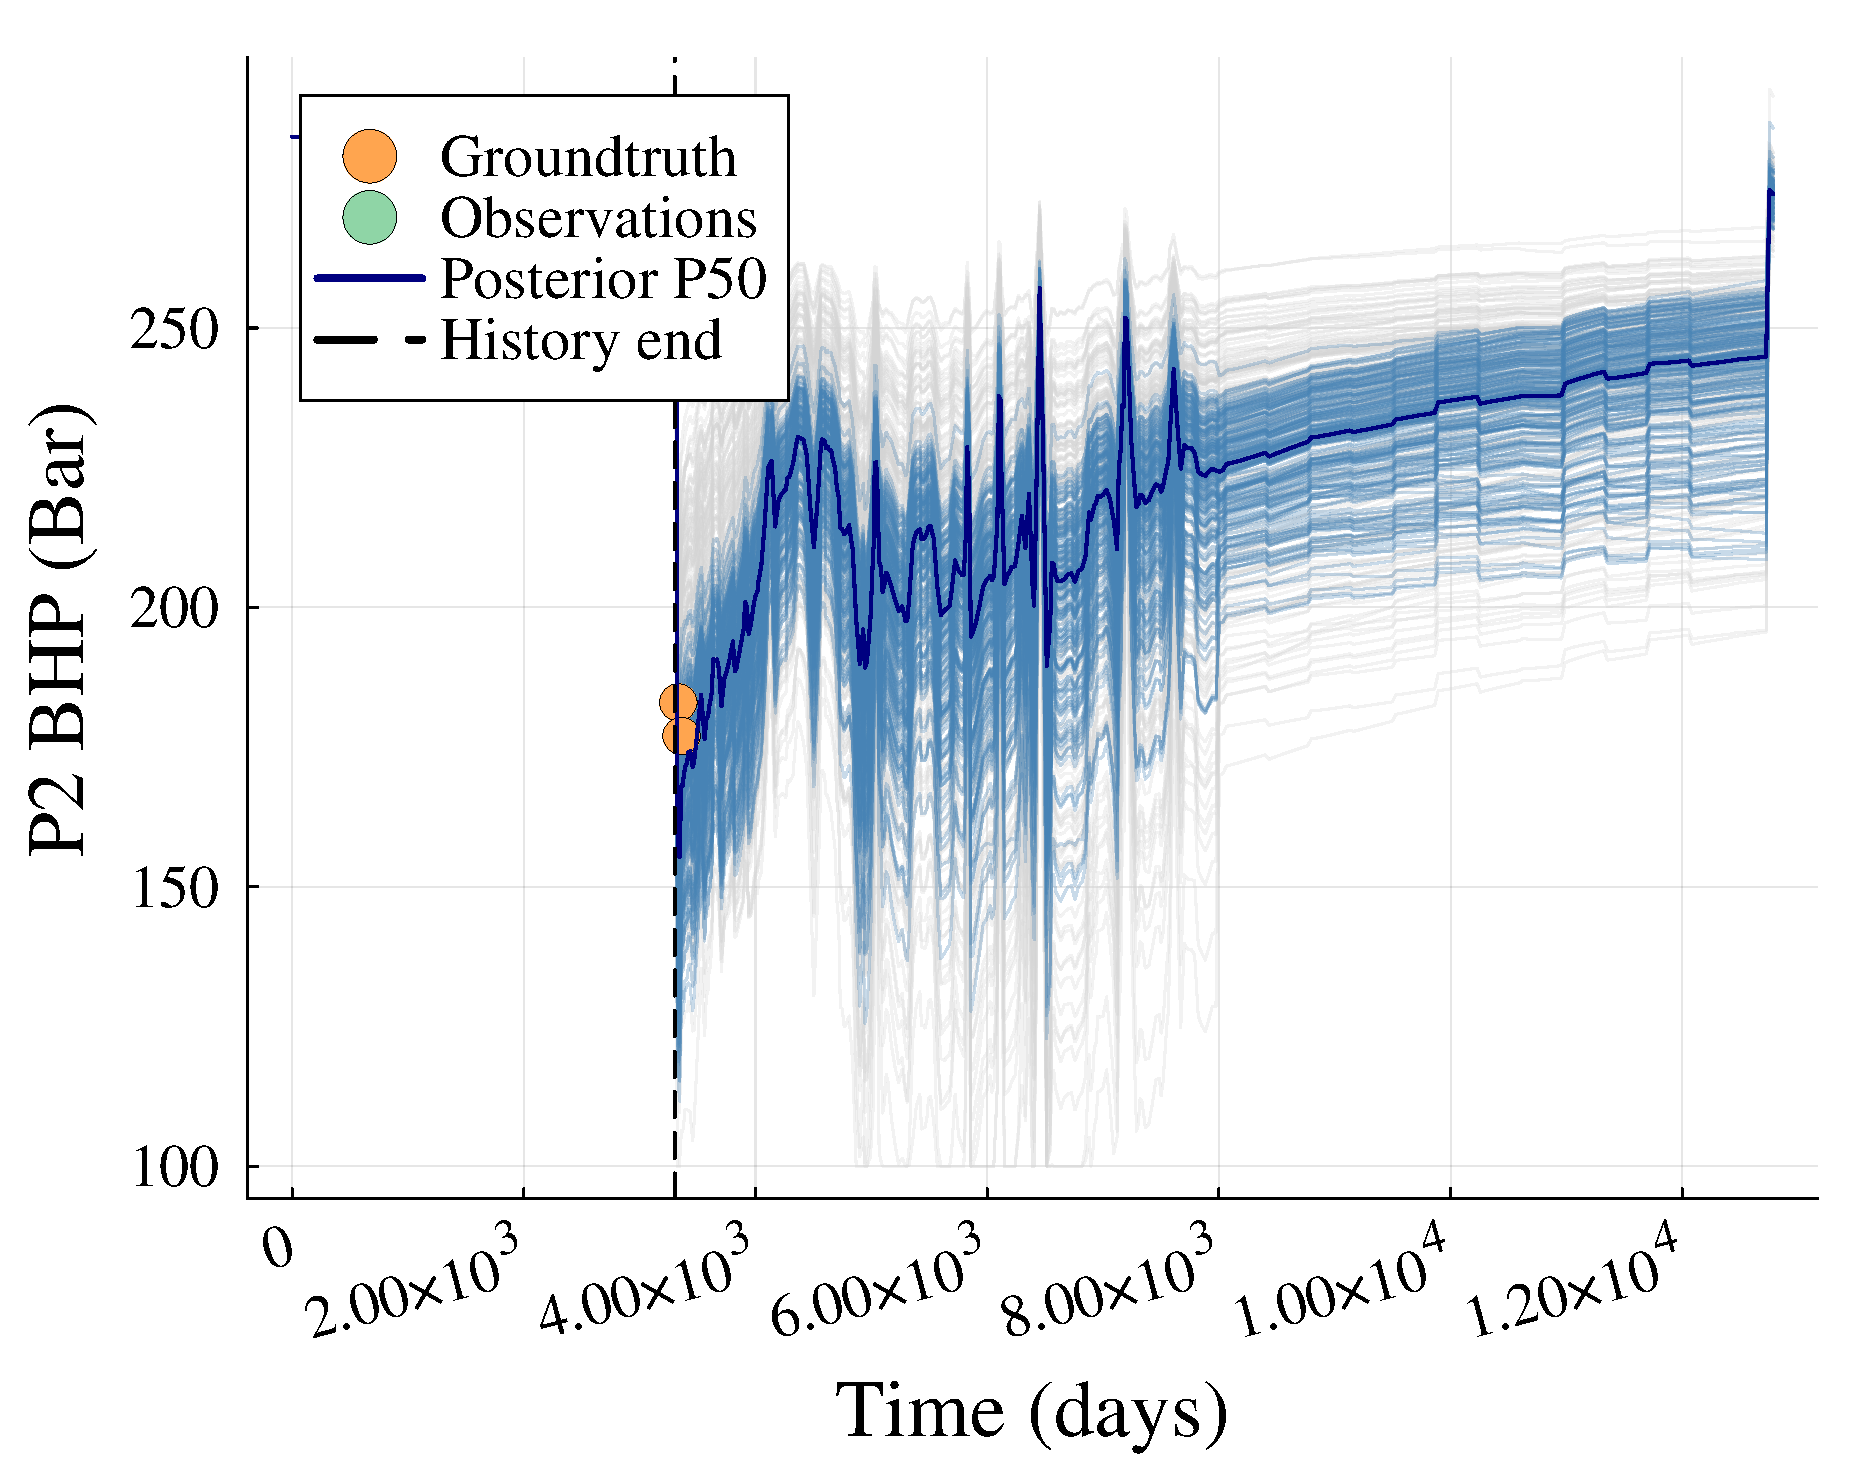
\includegraphics[width=0.775\linewidth]{figures/results/real_field/gt_0/noise_magnitude_0.01/n_iterations_1/localization_false/gating_true/gating_intensity_4.0/WELLS_P2_WBHP.pdf}
        \end{subfigure}
        \begin{subfigure}{.49\linewidth}\centering
            
\includegraphics[width=0.775\linewidth]{figures/results/real_field/gt_0/noise_magnitude_0.01/n_iterations_1/localization_false/gating_true/gating_intensity_4.0/WELLS_P11_WBHP.pdf}
        \end{subfigure}
        \begin{subfigure}{.49\linewidth}\centering
            
\includegraphics[width=0.775\linewidth]{figures/results/real_field/gt_0/noise_magnitude_0.01/n_iterations_1/localization_false/gating_true/gating_intensity_4.0/WELLS_P12_WBHP.pdf}
        \end{subfigure}
    \end{figure}
\end{frame}

\begin{frame}{Results}{Discussion}
    \begin{block}{Mild and small gating intensities versus standard DSI-ESMDA}
        Mild gating intensities (2 in the Egg and Olympus cases, 4 in the real field case) produced similar results 
        to the standard DSI-ESMDA for same localization configuration,
        while small gating (1 for the Egg case, 1 and 2 for the Olympus and real field cases)
        had worse coverages than the standard DSI-ESMDA.
    \end{block}
    \vfill
    \def\arraystretch{1.75}
    \begin{tabular}{rp{0.93\linewidth}}
        $\triangleright$ & 
        Gating intensity ``reverts'' the posterior to the prior.
        If the posterior given by the standard DSI-ESMDA is somewhere in that continuum,
        then it stands to reason that Gated DSI-ESMDA could approximate it simply by tuning the gating intensity.
    \\
        $\triangleright$ & 
        Since Gated DSI-ESMDA does away with observation data resampling,
        small gatings possibly underestimate uncertainty (i.e., likelihood covariance)
        at least when compared to standard DSI-ESMDA,
        producing posteriors that are not well-matched to data.
    \end{tabular}
\end{frame}